% -- Encoding UTF-8 without BOM
% -- XeLaTeX => PDF (BIBER)

\documentclass[]{cv-style}     % Add 'print' as an option into the square bracket to remove colours from this template for printing. 
                               % Add 'espanol' as an option into the square bracket to change the date format of the Last Updated Text
%\setdefaultlanguage{spanish}
%\sethyphenation[variant=spanish]{}{}  % Add words between the {} to avoid them to be cut 

\usepackage{graphicx}
\usepackage{csquotes}
\usepackage[document]{ragged2e}

\bibliography{bibliography}

\begin{document}

\header{Matteo}{Neri}{PhD candidate and Data Scientist}
\lastupdated

%----------------------------------------------------------------------------------------
% SIDEBAR SECTION  -- In the aside, each new line forces a line break
%----------------------------------------------------------------------------------------
\begin{aside}
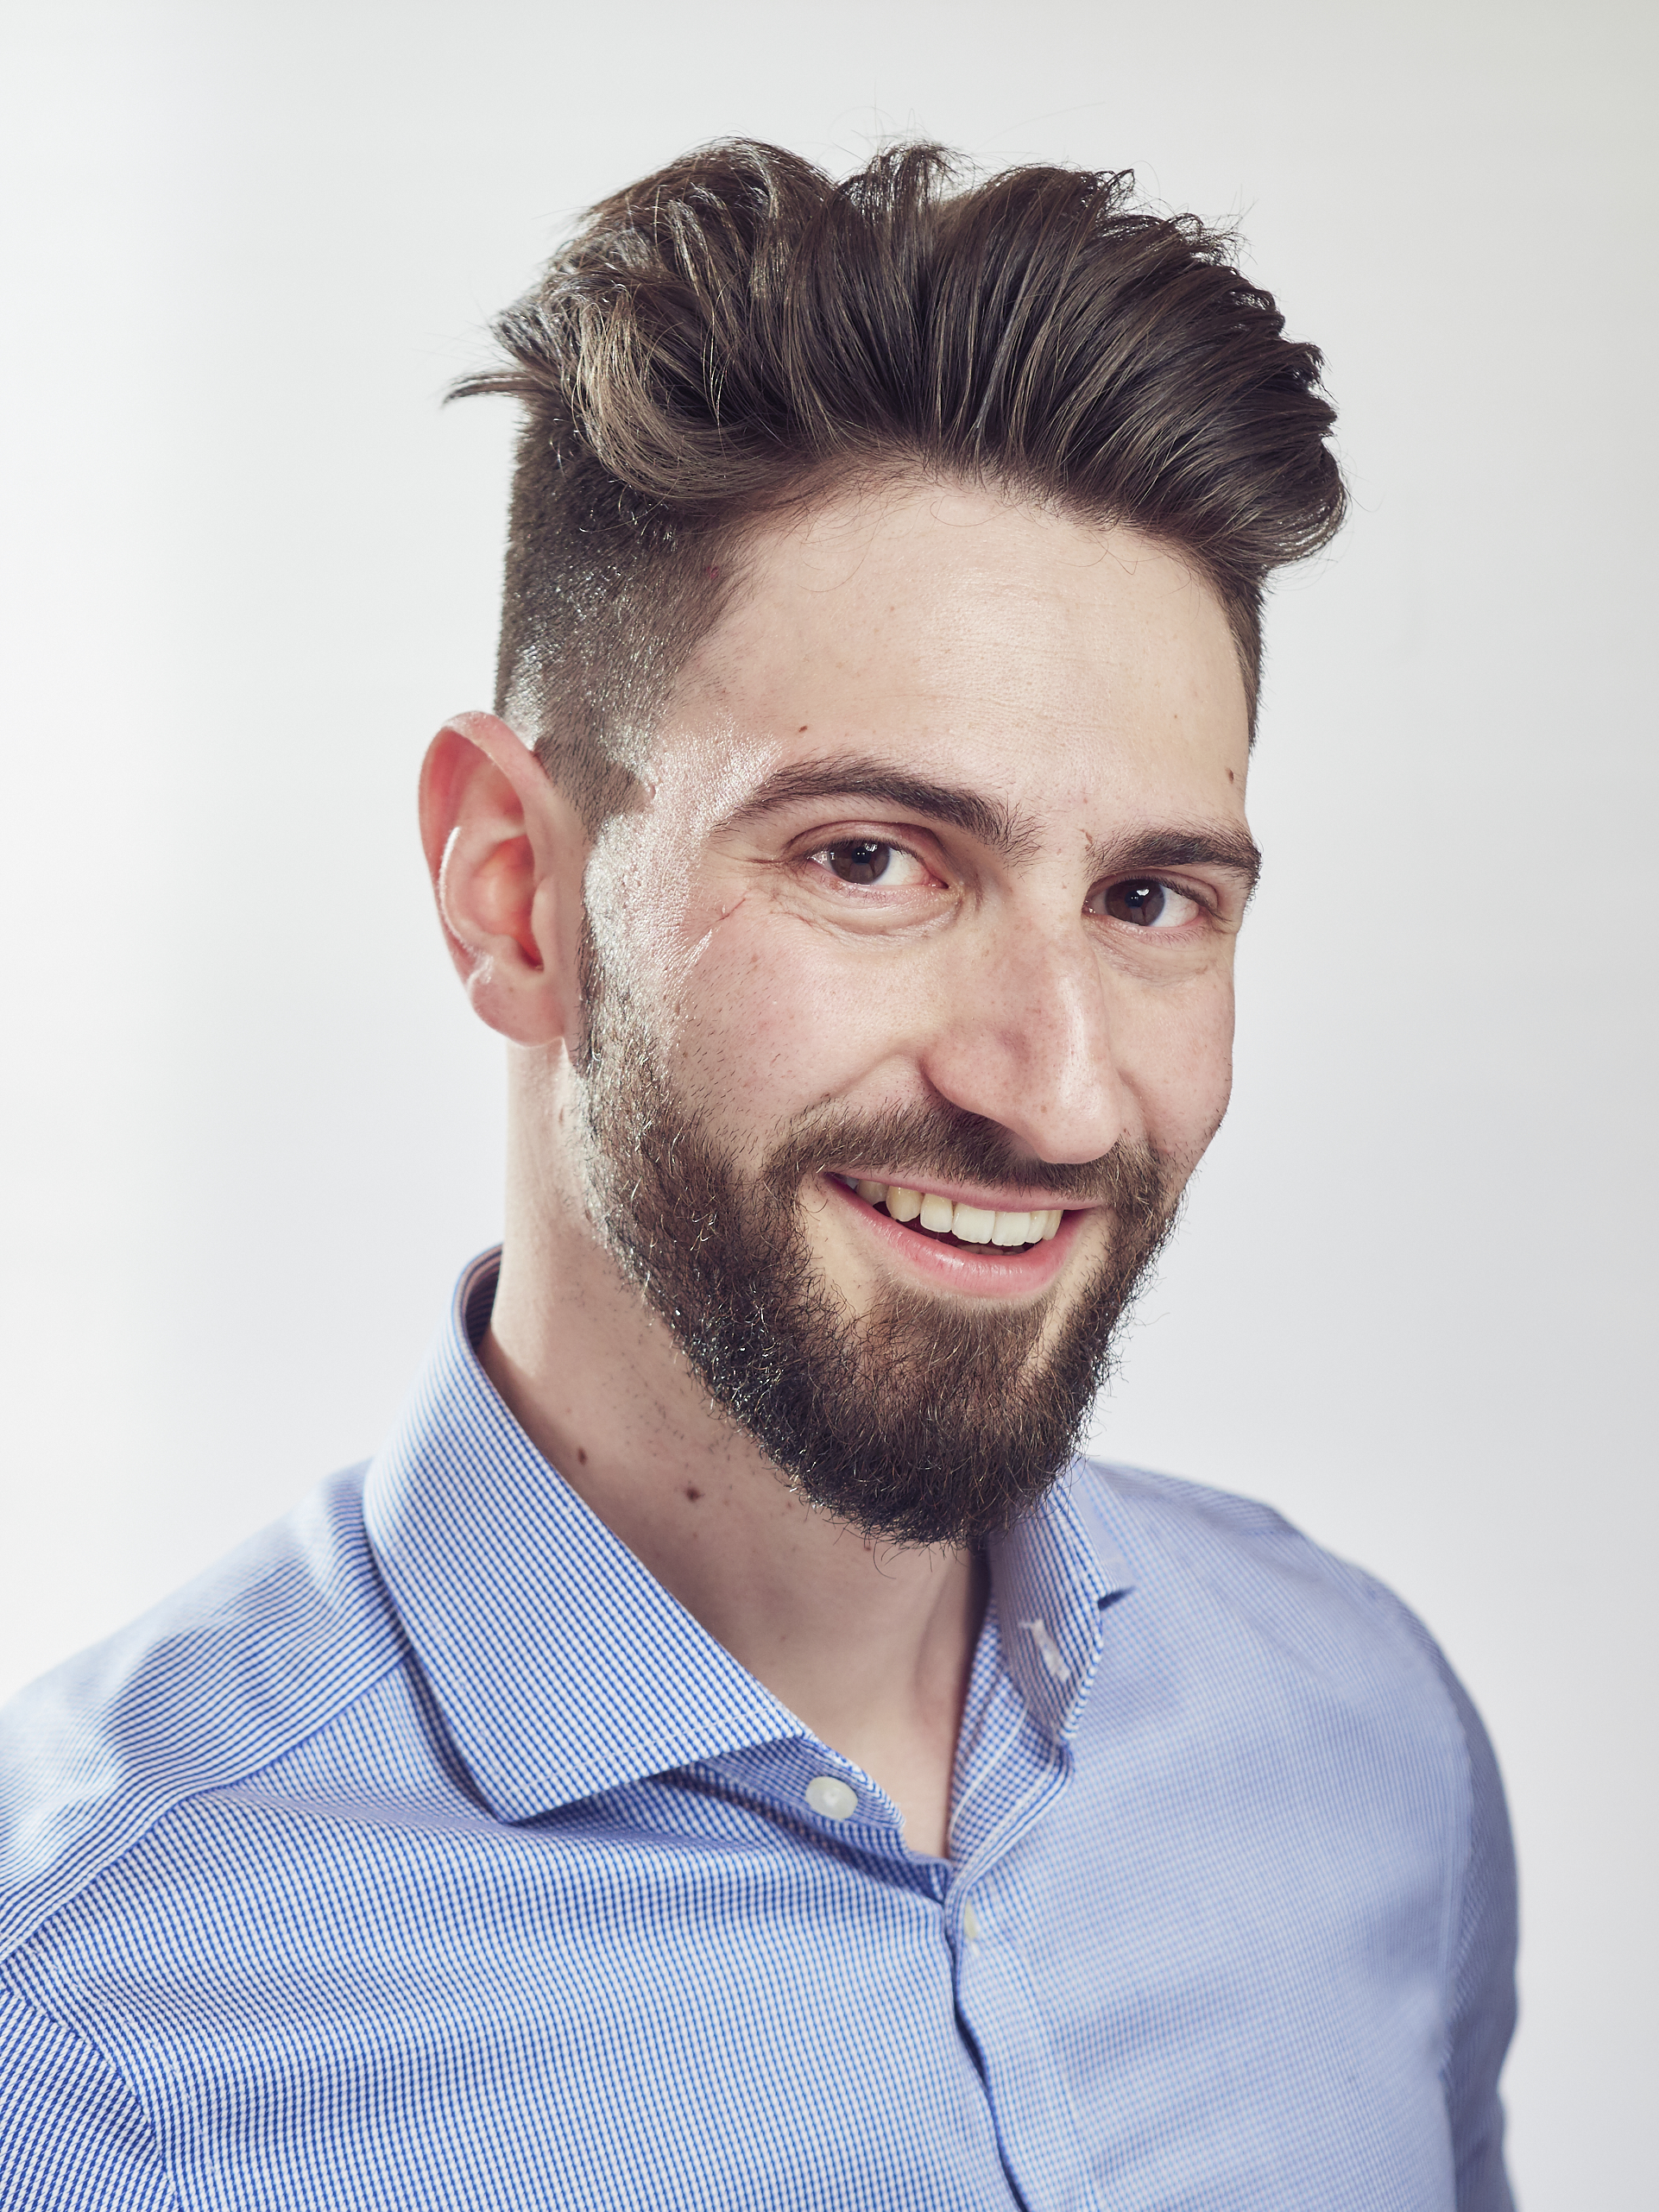
\includegraphics[scale=0.25]{FNA_Portraits_March_2019_902.jpg}
%
\section{contact}
Nador utca 11
Office 611, 6th floor
Pest 1051
Budapest, V. ker\"ulet
Hungary
%via Benedetta, 1
%48027 Solarolo (RA)
%Italy
~
+393289536548
~
\href{https://github.com/matteoneri}{github.com/matteoneri}
~
\href{mailto:nremtt@gmail.com}{nremtt@gmail.com}
\href{mailto:Neri_Matteo@phd.ceu.edu}{Neri\_Matteo@phd.ceu.edu}
%
\section{languages}
\it{italian}: mother tongue
\it{english}: language currently used
\it{spanish}: intermediate level
\end{aside}
%----------------------------------------------------------------------------------------
% EDUCATION
%----------------------------------------------------------------------------------------
\section{education}
\begin{entrylist}
\entry
{2017-Present}{PhD Candidate in Network Science}
{\href{http://www.ceu.edu}{Central European University}, Budapest, HU}{PhD candidate in Network Science.}
\entry
{2015-2017}
{M.Sc. - Physics of Complex Systems%\\
%M.SC. mathematical modeling for engineering
}
{%\href{https://www.sissa.it/}{SISSA},\href{http://www.ictp.it/}{ICTP},
%\href{http://www.polito.it/?lang=en}{PoliTO},
\href{https://www.universite-paris-saclay.fr/en}{Paris Saclay University}, Paris, FR
}
{\normalfont International master course in Physics of Complex Systems.\\
The courses are provided by a collaboration among SISSA, ICTP, Politecnico di Torino
and a consortium of universities from Paris (Paris Sud University, Pierre and Marie Curie University and Paris Diderot University).
Strong \href{http://www.lps.ens.fr/~benamar/sc/physics-of-complex-systems/}{knowledge} in statistical mechanics (and its application in different fields), inference, algorithms, complex networks, disordered systems, game theory, inference and learning.
}
%------------------------------------------------
\entry
{2011-2015}
{B.Sc magna cum laude - Physics}
{\href{http://http://www.unibo.it/en}{University of Bologna, Bologna, IT}}
{Majored in Physics, dissertation title:
\href{http://www.infn.it/thesis/PDF/getfile.php?filename=9796-Neri-triennale.pdf}
{``Studi di Data Popularity nell'analisi distribuita su Grid dell'esperimento CMS a LHC''}}
%------------------------------------------------
\entry
{2006-2011}
{High School Scientific Diploma}
{\href{http://www.liceotorricelli.it/}{Liceo Torricelli, Faenza (Italy)}}
{Specialization in mathematics and physics}
\end{entrylist}
%----------------------------------------------------------------------------------------
% EXPERIENCE SECTION
%----------------------------------------------------------------------------------------
\section{experiences}
\begin{entrylist}
\entry
{April 2018 - \\Present}
{Data Science Consultant}
{\href{http://www.fna.fi}{@ Finantial Networks Analytics}, London, UK}
{\footnotesize{\textbf{Main solution area: Financial Crime \& Conduct Risk.}}\\
FNA is a fast-growing, deep technology company and a leader in Regulatory and Supervisory
Technology. FNA's mission is to make the financial system safer and more efficient. FNA's SaaS Platform allows financial institutions to map and monitor complex financial networks and to simulate operational and financial risks. FNA’s clients include the world’s largest central banks, financial market infrastructures, and leading financial institutions.
}

\entry
{Winter Term\\2019}
{Teaching Assistant - Statistical Methods}
{\href{http://www.ceu.edu}{Network and Data Science Dep. @ CEU},
\begin{flushright}Budapest, HU
 \end{flushright}
}
{}
\entry
{Fall Term\\2018}
{Teaching Assistant - Scientific Python}
{\href{http://www.ceu.edu}{Math Department @ CEU},
\begin{flushright}Budapest, HU
 \end{flushright}
}
{}
\entry
{March -\\June 2017}
{Research Internship}
{\href{http://www.cmla.ens-cachan.fr/}{CMLA} @ \href{http://www.ens-cachan.fr/}{ENS Saclay}, Paris, FR}
{The purpose of the work was to analyze time-varying networks where Dynamic Resource Allocation Strategy has been adopted in order to treat the epidemic process in a high-resolution context. Considering evolving networks during epidemic control is an important step through real networks applications.}
\end{entrylist}
\begin{entrylist}
\entry
{July 2014 -\\March 2015}
{Research Internship}
{\href{http://home.infn.it/it/}{@ National Institute of Nuclear Physics (INFN)}, Bologna, IT}
{
I worked inside the CMS Collaboration (CMS is one of the four general purpose
    experiments at LHC at CERN) at one tool that intends to study the Run-1
    data-access patterns of the whole CMS experiment at Tier-2 level.
    The purpose of the work was to contribute to a project that aims to
    exploit the CMS data popularity to model the evolution of the CMS
data management towards a dynamic data management.
}
%\entry
%{July, 12th -\\July, 15th 2011}
%{\href{http://www.ducati.it/fondazione_ducati/index.do}{Fondazione Ducati}}
%{Bologna, Italy}
%{Summer School Fisica in Moto 2011}
%\entry
%{March 2011}
%{National Institute of Nuclear Physics (INFN)}
%{Bologna, Italy}
%{Masterclass Hands on Particle Physics}
\end{entrylist}

\section{schools and conferences}
\begin{entrylist}
\entry
{Jan 7th-11th\\2019}
{\href{http://bigdat2019.irdta.eu/}{International Winter School on Big Data}}
{University of Cambridge, Cambridge, UK}
{Research training event with a global scope aiming at updating participants on the most recent advances in the critical and fast developing area of big data}
\entry
{July 15th-21st\\2018}
{\href{https://sites.google.com/view/varennacs2018}{International Summer School Enrico Fermi on\\Computational Social Science and Complex Systems}}
{Varenna, IT}
{The Enrico Fermi Schools are a highly prestigious series of summer schools of the Italian Physical Society with a tradition of more than 60 years and with many Nobel laureates as lecturers.}
\entry
{April 12th-13th\\2018}
{\href{http://ibs-italy.org/?page_id=703&lang=en}{COSTNET Networking Biostatistics}}
{San Raffaele University, Milano, IT}
{Graphical models and Applications}
\entry
{March 15th-16th\\2018}
{\href{https://www.oxforduniversitystores.co.uk/conferences-events/statistics/statistics/costnet-sandpit-meeting}{COSTNET Sandpit Meeting}}
{University of Oxford, Oxford, UK}
{Exploring (massive) network data sets, Network Modelling, Network Inference and Prediction}
\entry
{June 19th-22nd\\2017}
{\href{https://regularize-in-paris.github.io/}{Structured Regularization for High-Dimensional Data Analysis\\Summer School}}
{Institut Henri Poincaré, Paris, FR}
{}
\end{entrylist}

%----------------------------------------------------------------------------------------
% TECHNICAL SKILLS
%----------------------------------------------------------------------------------------
\section{technical skills and expertise}
\par\vspace{.5\parskip}%
 {\color{gray}\headingfont Operating System}
 \begin{itemize}
  \item GNU-Linux
 \end{itemize}
 {\color{gray}\headingfont Programming Languages & Databases}
 \begin{itemize}
  \item Python [3+ years experience]
  \item C++ [4+ months]
  \item SQL (MariaDB)
 \end{itemize}
 {\color{gray}\headingfont Frameworks}
 \begin{itemize}
  \item ROOT
  \item spark
 \end{itemize}
 {\color{gray}\headingfont Other}
 {%\bodyfont\color{headercolor}
 \begin{itemize}
  \item elements of IT security and cryptography
  \item elements of functional programming
  \item elements of design patterns
 \end{itemize}
 }
 \par\vspace{.5\parskip}
 
\pagebreak
%----------------------------------------------------------------------------------------
% PUBBLICATIONS
%----------------------------------------------------------------------------------------
\section{pubblications}
\printbibsection{article}{article in international peer-reviewed journals} 
%----------------------------------------------------------------------------------------
% AWARDS SECTION
%----------------------------------------------------------------------------------------
\section{awards}
\par\vspace{.5\parskip}%
\begin{entrylist}
%------------------------------------------------
\entry
{2016-2017}
{IDEX Paris Saclay Scholarship - \euro 10,000}
{}
{}
%------------------------------------------------
\end{entrylist}
\end{document}
